\documentclass[conference]{IEEEtran}
\usepackage[T1]{fontenc}
\usepackage{cite}
\usepackage{amsmath,amssymb}
\usepackage{graphicx}
\usepackage{booktabs}
\usepackage{hyperref}
\usepackage{xcolor}
\usepackage{microtype}
\usepackage{flushend}
% Moderate float spacing (6-page target; references on final page).
\setlength{\textfloatsep}{5pt plus 2pt minus 2pt}
\setlength{\floatsep}{5pt plus 2pt minus 2pt}
\setlength{\intextsep}{7pt plus 3pt minus 3pt}
\setlength{\abovecaptionskip}{2pt}
\setlength{\belowcaptionskip}{1pt}
\newcommand{\figw}{0.84\columnwidth}

\title{Robust AI-Image Detection Using a Classical Baseline and a Transfer-Learned CNN}

\author{
\IEEEauthorblockN{Daniel Harapiak}
\IEEEauthorblockA{
Department of Computer Science\\
Western University\\
London, ON, Canada\\
dharapia@uwo.ca
}
\and
\IEEEauthorblockN{Aydan Karmali}
\IEEEauthorblockA{
Department of Computer Science\\
Western University\\
London, ON, Canada\\
akarma5@uwo.ca
}
\and
\IEEEauthorblockN{Maximilian Cope}
\IEEEauthorblockA{
Department of Computer Science\\
Western University\\
London, ON, Canada\\
mcope4@uwo.ca
}
}

\begin{document}
\maketitle

\begin{abstract}
We study binary AI-image detection where clean-benchmark scores can mislead when images are compressed or resized. A logistic-regression baseline on handcrafted features and a transfer-learned ResNet-18 are compared on a balanced GenImage subset (22,400/4,800/4,800 train/val/test) with fixed manifests, saved configs, and traceable artifacts. We report accuracy, precision, recall, F1, ROC-AUC, and confusion behavior. We stress-test the CNN under JPEG (Q85 to Q40) and resize (0.75/0.5). Clean test results: baseline 0.7142 accuracy / 0.7211 F1; CNN 0.9465 / 0.9452; under JPEG Q40, CNN F1 falls to 0.5945 with a large shift toward missed AI images. Contribution: a compact workflow pairing fair clean comparison with degradation-aware, auditable failure analysis. Main takeaway: strong clean performance does not imply robustness to everyday post-processing. Future work: broader generator coverage, robustness-aware training, and calibrated operating points.
\end{abstract}

\begin{IEEEkeywords}
AI image detection, deep learning, computer vision, transfer learning, robustness, logistic regression, ResNet
\end{IEEEkeywords}

\section{Introduction}
Recent text-to-image generators have made synthetic image content widely accessible. Modern pipelines span GAN-based methods~\cite{goodfellow2014gan,karras2020stylegan2} and diffusion-based methods~\cite{ho2020ddpm,rombach2022ldm}, and realism has improved rapidly. As quality rises, manual inspection becomes less reliable and automated forensics-style detection grows in importance for dataset curation, moderation support, and integrity checks~\cite{verdoliva2020mediaforensics}.

Prior work shows detector performance is sensitive to data distribution, generator family, and post-processing~\cite{wang2020cnn,chai2020makes}: a model can score well on a clean benchmark yet degrade under compression, resizing, or unseen generators. That gap between benchmark and deployment means evaluation should not rely on a single headline accuracy score.

This work addresses binary classification: label an image as natural (real) or AI-generated. We compare a classical handcrafted-feature baseline to a transfer-learned CNN on identical splits, then stress-test robustness with JPEG and resize (transformations common in real sharing pipelines).

Many studies emphasize clean-split accuracy and give less prominence to how errors shift under degradation. We make robustness visible alongside clean metrics and tie numbers to confusion behavior. Contributions: reproducible classical vs.\ deep comparison with saved configs and plots; fixed manifests for fair splits; explicit JPEG/resize protocol; analysis of failure modes. On clean data the CNN leads (0.9465 vs.\ 0.7142 accuracy) but drops under heavy JPEG, so deployment must balance clean separability against post-processing sensitivity.

Research goals: \textbf{O1} build a reproducible pipeline with fixed train/validation/test splits; \textbf{O2} compare classical features plus logistic regression to a transfer-learned ResNet under the same conditions; \textbf{O3} quantify robustness under JPEG compression and resolution reduction.

The report is organized as follows: Section II reviews related work; Section III describes methods; Section IV presents results; Section V concludes with lessons and future work.

From an evaluation standpoint, we treat the CNN as the primary detector for stress testing because it is the stronger clean model and therefore the more plausible candidate for deployment on this benchmark; the classical baseline remains important as an interpretable lower bound and sanity check on the same labels and file lists.

\section{Background and Related Work}
\subsection{AI-image detection and dataset choice}
AI-image detection has become an important computer vision problem due to rapid improvements in generative models. The GenImage benchmark is designed for this task and is widely used for evaluating detector generalization across generators and settings~\cite{zhu2023genimage}. To keep the project computationally manageable while preserving class balance and reproducibility, this implementation uses two generators (BigGAN and Midjourney) and fixed split manifests. This follows prior evidence that cross-generator setup choices strongly affect reported detector performance~\cite{zhu2023genimage,ojha2023universal}.

GenImage yields generator-aware splits; training on two generators alone does not ensure cross-generator generalization. We nevertheless obtain a controlled setting where real vs.\ AI labels are balanced and file lists are frozen, which supports repeatable training and fair comparison between the classical pipeline and the CNN.

\subsection{Classical versus deep approaches}
Classical approaches often rely on handcrafted frequency and statistical cues with linear or kernelized classifiers. They are easier to interpret and cheaper to train, but usually underperform deep models on complex visual distributions.

Deep CNNs, especially transfer-learned ResNet variants, are strong baselines for image classification and align with course expectations for architecture and training~\cite{he2016resnet,torchvisiondocs}. Fake-image detection literature reports that semantic and frequency-domain cues can both matter depending on generator and test regime~\cite{frank2020leveraging,wang2020cnn}. Deep models can exploit richer cues yet may latch onto shortcuts that fail when inputs are degraded; we compare both families on one split to relate clean gains to robustness behavior.

\subsection{Robustness and distribution shift in prior work}
Detectors can fail under compression, resampling, and generator shift~\cite{wang2020cnn,chai2020makes,ojha2023universal}. We therefore report condition-specific metrics (not only aggregate clean scores) using JPEG quality steps and resize factors chosen to mimic common user-side processing.

\subsection{Research gap addressed}
We target two issues: over-reliance on clean-only reporting, and limited auditability of how results were obtained. The project uses fixed splits, artifact-traceable classical vs.\ CNN runs, and explicit robustness tests under JPEG and resize.

\section{Methods}
\label{sec:methods}
\subsection{Research objectives and significance}
\textbf{O1}: build a reproducible pipeline using fixed split manifests and saved run artifacts. \textit{Significance}: this supports reliable verification of how metrics were produced.\\
\textbf{O2}: run a fair comparison between a classical baseline and a transfer-learned CNN under the same split conditions. \textit{Significance}: this isolates modeling effects from data-split differences.\\
\textbf{O3}: quantify deployment risk under image-quality shifts using controlled JPEG and resize tests. \textit{Significance}: this links benchmark performance to likely real-use behavior where post-processing is common.

\subsection{Dataset and splits}
The project uses a GenImage-derived subset with two generators, BigGAN and Midjourney, and two classes, real (nature) and ai. The combined split counts are 22,400 for training, 4,800 for validation, and 4,800 for testing.

This subset choice was made because GenImage is task-aligned and generator-aware, while the selected size remains feasible under course compute limits without sacrificing class balance. Dataset splits are defined using fixed manifest tables and consumed by a dataset loader that performs on-the-fly image loading from file paths with associated binary labels.

Labels are verified at load time; any missing path is treated as an error so that silent subsampling cannot skew comparisons between models.

\begin{table}[htbp]
\caption{Per-Generator Split Counts (per class)}
\label{tab:split-counts}
\centering
\begin{tabular}{lccc}
\toprule
Split & BigGAN (ai/real) & Midjourney (ai/real) & Combined \\
\midrule
Train & 5600 / 5600 & 5600 / 5600 & 22400 \\
Val & 1200 / 1200 & 1200 / 1200 & 4800 \\
Test & 1200 / 1200 & 1200 / 1200 & 4800 \\
\bottomrule
\end{tabular}
\end{table}

\subsection{Research question and hypothesis}
The guiding research question is: \emph{How much does a transfer-learned CNN improve AI-image detection performance over a classical handcrafted-feature baseline, and how stable is that improvement under common degradations?}

Hypothesis H1: the CNN will significantly outperform the baseline on clean test data.\\
Hypothesis H2: both models, especially the CNN, will lose performance under stronger JPEG and resize perturbations.

Robustness under common transforms matters as much as clean accuracy for practical use.

\subsection{Model 1: Classical baseline}
The baseline extracts handcrafted image features and trains a logistic regression classifier with standardization. The feature set includes a grayscale histogram (32 bins), RGB channel means and standard deviations, gradient magnitude statistics, FFT-derived low/high-frequency energy statistics, and an entropy feature. Histogram and RGB moments capture coarse color and intensity structure; gradients summarize edges and texture energy; FFT bands probe frequency-domain energy splits that often differ between natural photographs and synthesized content; entropy summarizes global complexity. Together they form a compact vector that is cheap to compute and inspect relative to a deep embedding.

The classifier is implemented as \texttt{StandardScaler + LogisticRegression (lbfgs)}.
In the baseline configuration, logistic regression used \texttt{C = 1.0} and \texttt{max\_iter = 3000}, with predictions generated using a fixed decision threshold of \texttt{0.5}.

\subsection{Model 2: Transfer-learned CNN}
The deep model is a transfer-learned ResNet-18 binary classifier~\cite{he2016resnet}. This choice was made because ResNet-18 is a standard, course-aligned architecture with strong transfer-learning performance at moderate computational cost, which supports fair comparison without overengineering. The final fully-connected layer is replaced with one output logit and trained using BCEWithLogitsLoss. The main settings are image size $224 \times 224$, 8 epochs, batch size 48, learning rate $3 \times 10^{-4}$, weight decay $1 \times 10^{-5}$, and decision threshold 0.5.

Training applies resize to $224$, random horizontal flip ($p=0.5$), and ImageNet normalization; evaluation uses the same resize and normalization without flipping. Validation F1 selects the best checkpoint.

\subsection{Implementation strategy}
End-to-end workflow: manifest files drive CSV splits; we train and evaluate the baseline, then train the CNN and keep the validation-F1-best checkpoint; robustness evaluation runs on clean, JPEG, and resize conditions; optional inference supports ad-hoc images. Each run writes \texttt{config\_used.yaml}, \texttt{metrics.json}, plots, per-image predictions, and misclassification samples under timestamped directories so every figure and number can be traced to a configuration.

\subsection{Evaluation metrics and robustness protocol}
For both models we report precision, recall, and F1:
\begin{align}
\text{Precision} &= \frac{TP}{TP+FP}, \quad \text{Recall}=\frac{TP}{TP+FN}, \nonumber\\
\text{F1} &= 2\cdot\frac{\text{Precision}\cdot\text{Recall}}{\text{Precision}+\text{Recall}}.
\end{align}
We report accuracy, confusion matrices, ROC-AUC (when both classes appear), and per-image predictions. F1 highlights error trade-offs when missed AI images matter; ROC-AUC summarizes ranking across thresholds. CNN robustness uses JPEG Q85/Q60/Q40 and resize 0.75/0.5 (downsample then upsample to $224\times224$). The classical baseline is evaluated on the clean test split in full; the degradation ladder is applied to the CNN to keep the report focused on the model most likely to be used in practice while still documenting where performance collapses. Plots and tables for this study were generated with Matplotlib from the saved JSON metrics. Metrics derive from saved splits and run artifacts~\cite{sklearnlogreg,fawcett2006roc}.

\subsection{Threats to validity}
The detector is trained on BigGAN and Midjourney only, so generalization to other generators (including newer diffusion or proprietary APIs) is expected to be weaker than in-distribution performance. Hyperparameter search was limited and we report single runs per configuration, which is typical for a course project but leaves variance unquantified.

Resizing all inputs to a common size is standard for the CNN and baseline comparison, yet it may suppress fine-grained, resolution-dependent artifacts. That trade-off is unavoidable for a controlled apples-to-apples study but should be remembered when interpreting cross-generator claims.

\section{Results and Analysis}
\subsection{Clean model comparison}
Table~\ref{tab:clean-results} summarizes test metrics for baseline and CNN.

\begin{table}[htbp]
\caption{Clean Test-Set Comparison}
\label{tab:clean-results}
\centering
\setlength{\tabcolsep}{4.5pt}
\begin{tabular}{lccccc}
\toprule
Model & Acc. & Prec. & Recall & F1 & ROC-AUC \\
\midrule
Baseline & 0.7142 & 0.7040 & 0.7392 & 0.7211 & 0.7951 \\
CNN (ResNet-18) & 0.9465 & 0.9685 & 0.9229 & 0.9452 & 0.9887 \\
\bottomrule
\end{tabular}
\end{table}

The CNN substantially outperforms the classical baseline on all clean test metrics (Table~\ref{tab:clean-results}), which aligns with transfer-learned representations capturing richer multi-scale structure than fixed handcrafted summaries. The baseline still reaches moderate ROC-AUC, indicating that simple statistics carry signal, but not enough to match the CNN on this split.

Figures~\ref{fig:baseline-cm} and \ref{fig:baseline-roc} illustrate baseline behavior: confusion is more evenly spread and the ROC curve is shallower than for the CNN, consistent with Table~\ref{tab:clean-results}.

\begin{figure}[htbp]
\centerline{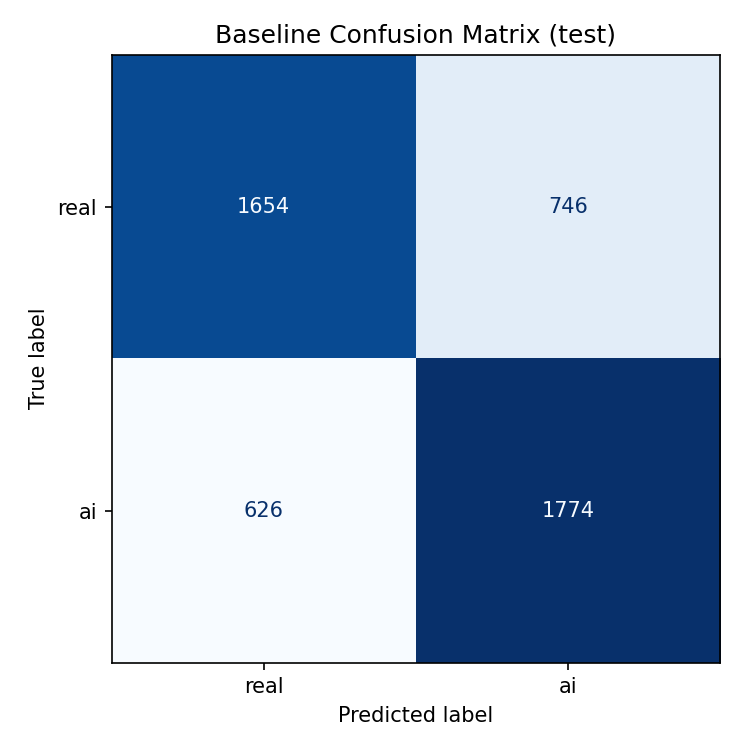
\includegraphics[width=\figw]{../report_handoff/plots+metrics/baseline/confusion_matrix_test.png}}
\caption{Baseline confusion matrix on clean test set.}
\label{fig:baseline-cm}
\end{figure}

\begin{figure}[htbp]
\centerline{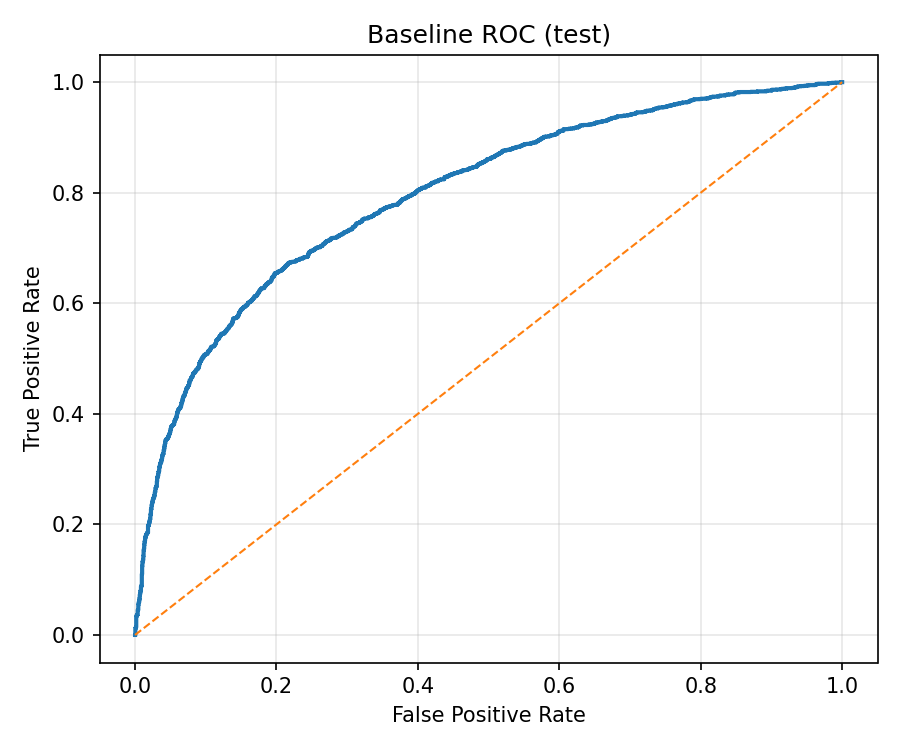
\includegraphics[width=\figw]{../report_handoff/plots+metrics/baseline/roc_curve_test.png}}
\caption{Baseline ROC curve on clean test set.}
\label{fig:baseline-roc}
\end{figure}

\subsection{CNN training dynamics}
Figure~\ref{fig:train-history} shows training and validation loss and metrics across eight epochs. Loss decreases steadily and validation F1 rises early, then levels off; we do not observe prolonged under-fitting that would suggest the CNN advantage is purely from insufficient training budget.

\begin{figure}[htbp]
\centerline{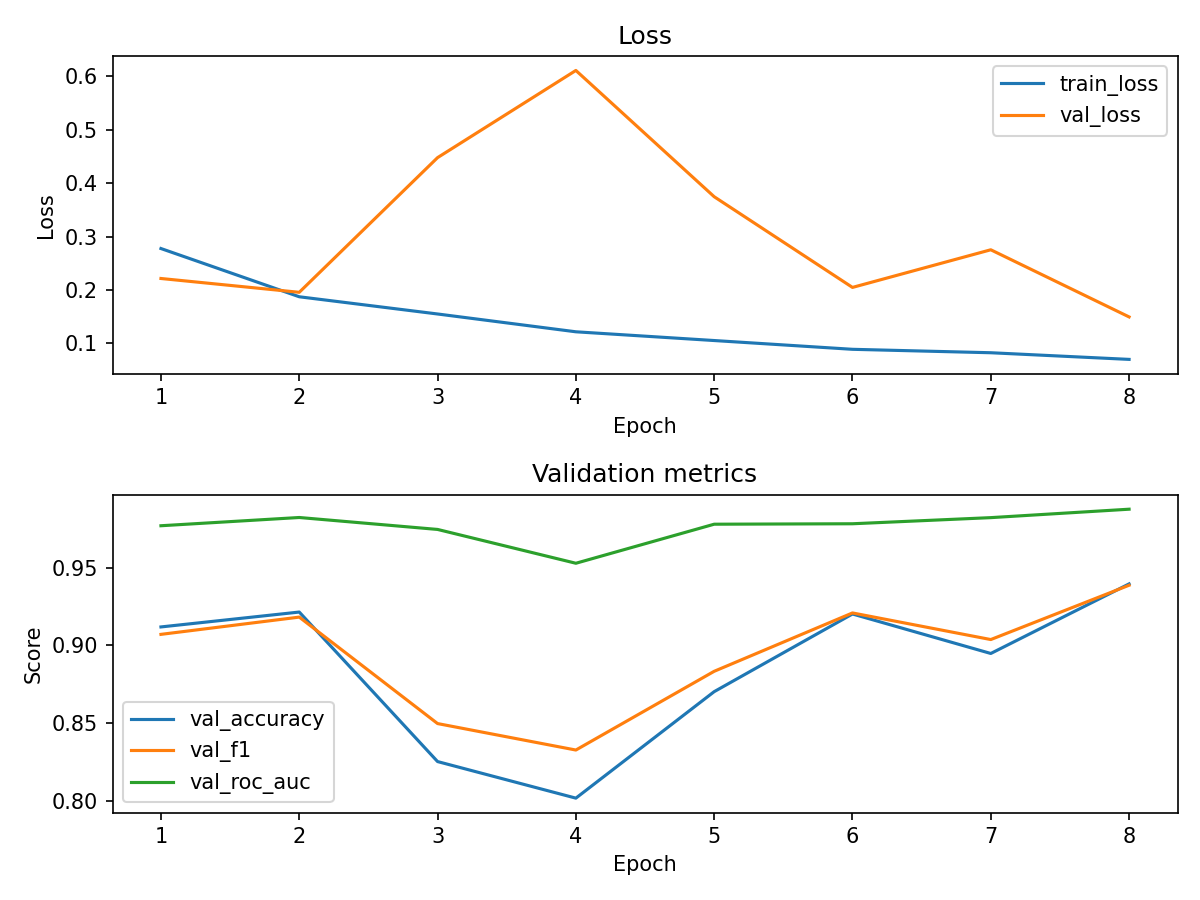
\includegraphics[width=\figw]{../report_handoff/plots+metrics/cnn/train_history.png}}
\caption{CNN training and validation history across epochs.}
\label{fig:train-history}
\end{figure}

\subsection{Confusion matrix and ROC interpretation}
On clean data the CNN (Figures~\ref{fig:cnn-cm}, \ref{fig:cnn-roc}) exhibits strong class separation and a high ROC-AUC, reflecting the margin visible in Table~\ref{tab:clean-results}. High clean ranking does not imply robustness to post-processing; Section~\ref{sec:robust} examines JPEG and resize effects.

\begin{figure}[htbp]
\centerline{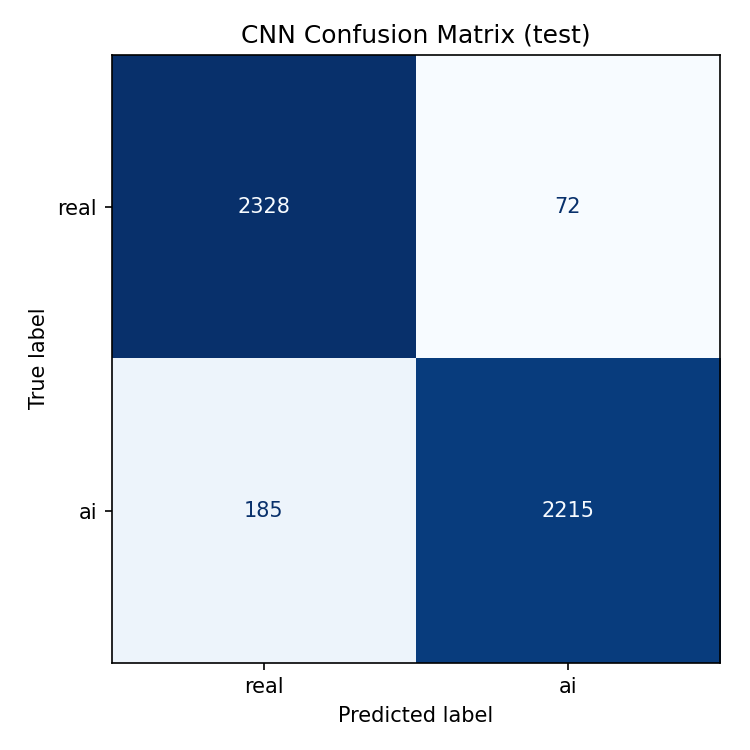
\includegraphics[width=\figw]{../report_handoff/plots+metrics/cnn/confusion_matrix_test.png}}
\caption{CNN confusion matrix on clean test set.}
\label{fig:cnn-cm}
\end{figure}

\begin{figure}[htbp]
\centerline{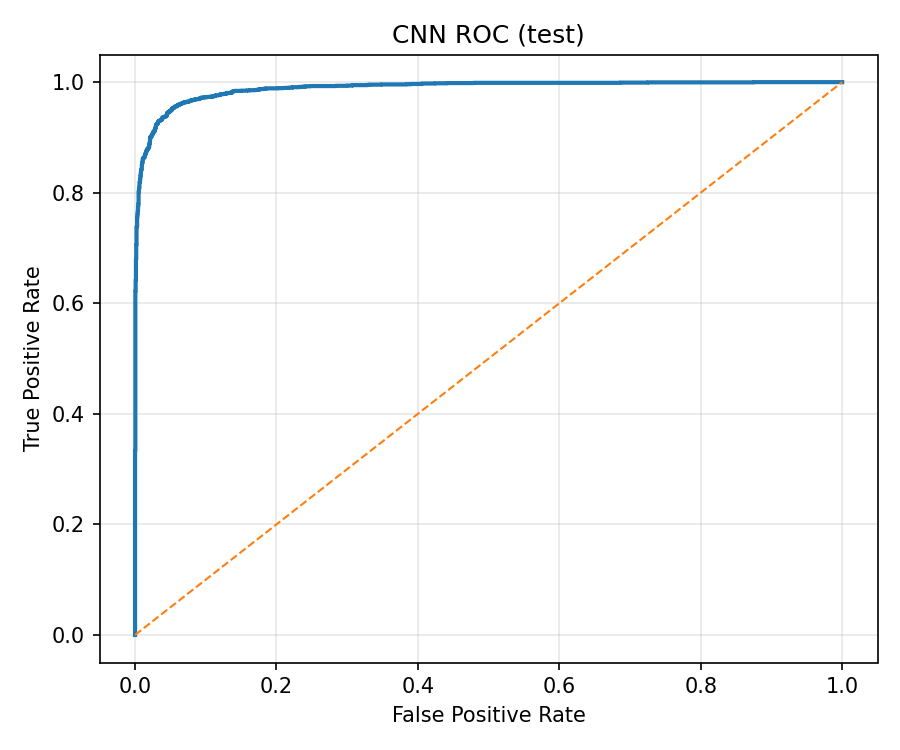
\includegraphics[width=\figw]{../report_handoff/plots+metrics/cnn/roc_curve_test.png}}
\caption{CNN ROC curve on clean test set.}
\label{fig:cnn-roc}
\end{figure}

\subsection{Robustness results}
\label{sec:robust}
Table~\ref{tab:robust-results} summarizes CNN robustness.

\begin{table}[htbp]
\caption{CNN Robustness Across Degradations}
\label{tab:robust-results}
\centering
\begin{tabular}{lccc}
\toprule
Condition & Accuracy & F1 & ROC-AUC \\
\midrule
Clean & 0.9465 & 0.9452 & 0.9887 \\
JPEG Q85 & 0.7931 & 0.7501 & 0.9159 \\
JPEG Q60 & 0.7388 & 0.6596 & 0.8830 \\
JPEG Q40 & 0.7050 & 0.5945 & 0.8728 \\
Resize 0.75 & 0.9006 & 0.9024 & 0.9619 \\
Resize 0.5 & 0.7521 & 0.7763 & 0.8209 \\
\bottomrule
\end{tabular}
\end{table}

Performance remains relatively strong under mild resizing and JPEG Q85, but heavier JPEG and stronger downscaling erode accuracy and F1, with recall suffering in particular. That pattern suggests the model relies partly on cues that compression and aggressive resampling remove or blur.

Interpreting Table~\ref{tab:robust-results} by condition: the JPEG ladder shows a monotonic decline from Q85 to Q40, with the steepest F1 drop between moderate and low quality, consistent with high-frequency cues being progressively quantized away. Resize 0.75 largely preserves F1 ($\approx$0.90), whereas resize 0.5 cuts ROC-AUC to 0.8209, indicating that aggressive downsampling destroys detail the network had used for discrimination even after upsampling back to network input size. Together, these curves argue that typical social-media compression is a more severe threat than modest resolution change for this architecture on this data.

Condition tags follow \texttt{eval\_config.yaml} (e.g., \texttt{clean}, \texttt{jpeg\_q40}, \texttt{resize\_0p5}); each run produces metrics and plots. Under Q40, false negatives on the AI class dominate: recall falls from 0.9229 (clean) to 0.4325 while precision stays high, so the system increasingly misses synthetic content, which is often worse for moderation than extra false alarms. Figures~\ref{fig:eval-table} and \ref{fig:eval-cm-jpeg40} summarize the degradation table and the Q40 confusion matrix.

\begin{figure}[htbp]
\centerline{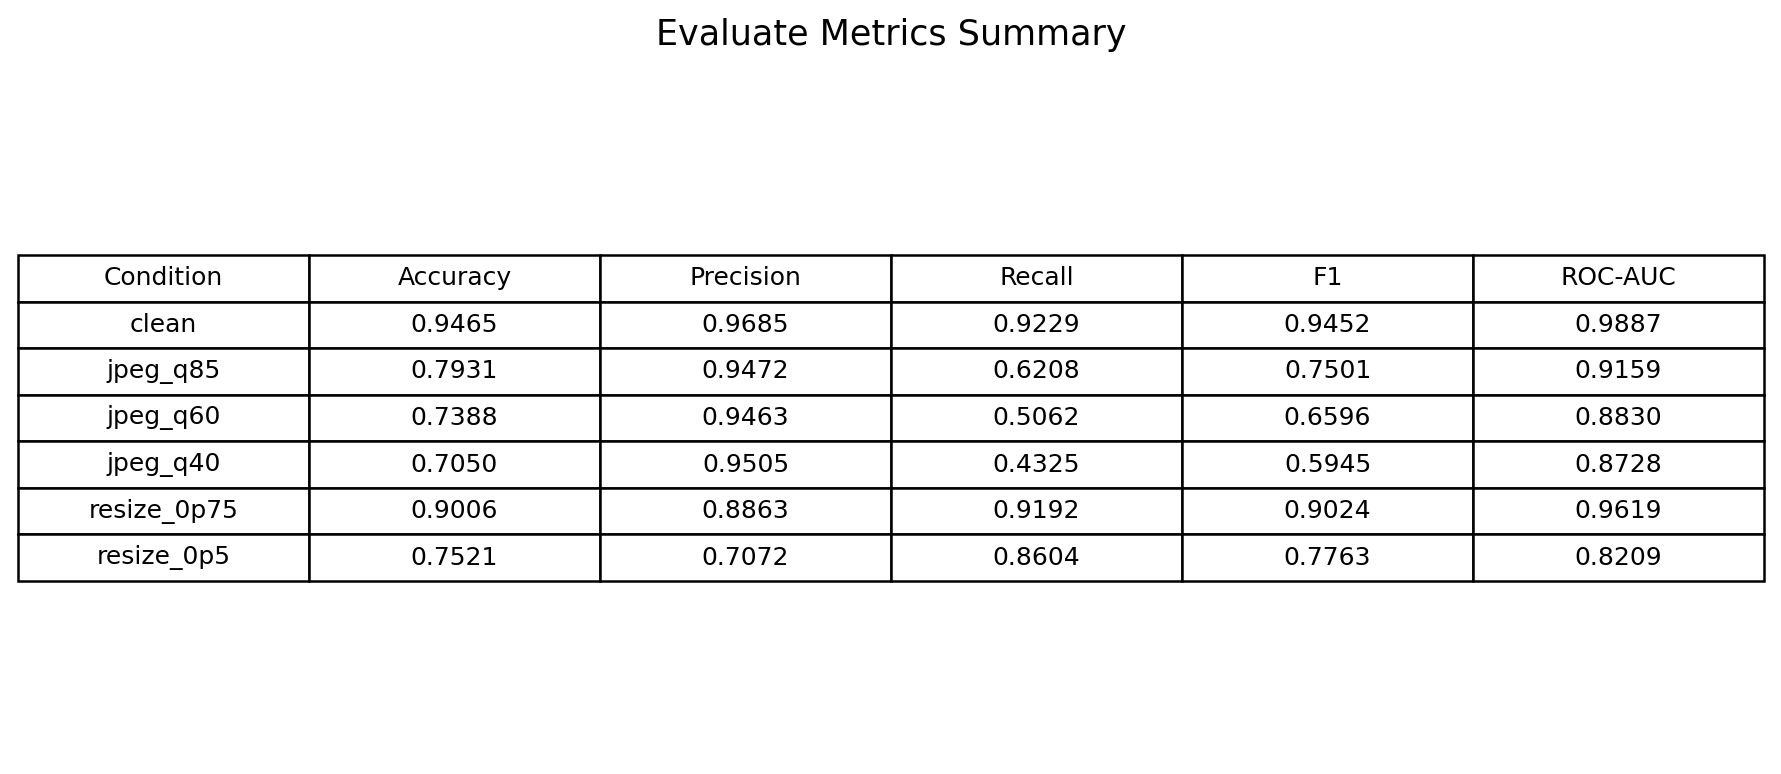
\includegraphics[width=\figw]{../report_handoff/plots+metrics/evaluate/evaluate_metrics_table.png}}
\caption{Evaluation summary table across clean and degraded conditions.}
\label{fig:eval-table}
\end{figure}

\begin{figure}[htbp]
\centerline{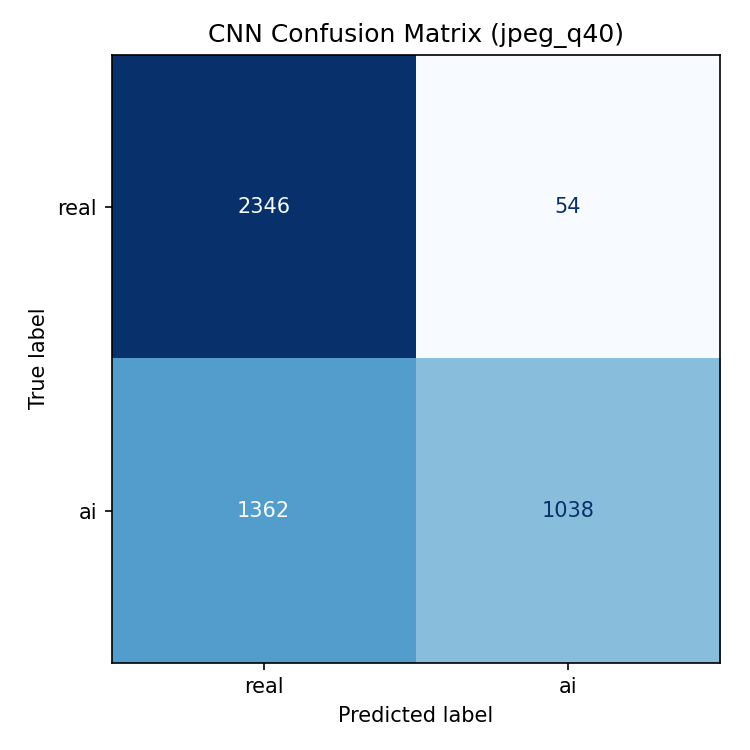
\includegraphics[width=\figw]{../report_handoff/plots+metrics/evaluate/confusion_matrix_jpeg_q40.png}}
\caption{CNN confusion matrix under heavy JPEG compression (Q40).}
\label{fig:eval-cm-jpeg40}
\end{figure}

\subsection{Discussion}
\textbf{H1} is supported: the CNN clearly outperforms the baseline on clean test data. \textbf{H2} is supported as well: both families would suffer under degradation, and the CNN's large clean margin narrows under heavy JPEG, so headline clean metrics understate operational risk when users recompress images.

These conclusions are tied to our GenImage subset and two-generator training. Generalization to other families and to post-processing not tested here should be treated cautiously, consistent with broader findings on cross-generator and robustness limits~\cite{zhu2023genimage,ojha2023universal,chai2020makes}.

For deployment-oriented readers, the practical implication is to pair any reported clean accuracy with at least a small battery of degradation tests that match the application's distribution (e.g., thumbnail sizes and typical JPEG quality). A detector that is only validated on pristine benchmark crops may appear ``ready'' while failing on the compressed content users actually share.

We do not tabulate a full JPEG/resize ladder for the classical baseline because it already trails the CNN on clean data; the operational question for moderation-style use is how the stronger model behaves under degradation, and the stress tests above target that model. A follow-up could still plot baseline vs.\ CNN under the same degradations to quantify how much of the gap closes when cues are destroyed.

\section{Conclusion and Future Work}
\subsection{Conclusion}
This work studied binary AI-image detection with a reproducible pipeline on a balanced GenImage subset (BigGAN and Midjourney), comparing a logistic-regression baseline on handcrafted features to a transfer-learned ResNet-18 under identical splits and evaluation code paths.

Relative to Section~\ref{sec:methods}, \textbf{O1} is satisfied: fixed manifests and saved configs/metrics/plots make each stage auditable. \textbf{O2} is satisfied: the CNN substantially outperforms the classical model on clean test data (Table~\ref{tab:clean-results}), supporting the value of deep transfer features for separability on this benchmark. \textbf{O3} is satisfied in the sense that robustness is explicitly quantified: while mild JPEG and resize leave the CNN usable, aggressive compression (e.g., Q40) drives F1 to 0.5945 and shifts errors toward missed AI images, which is often the more harmful failure mode in practice.

Hypothesis \textbf{H1} (CNN ahead on clean data) and \textbf{H2} (both models, especially the CNN, degrade under stronger degradations) are supported. The broader lesson is methodological: clean accuracy alone is not enough for real-world use when users routinely recompress or rescale media; reporting robustness curves and confusion behavior under degradation is as important as reporting a single test-set score. At the same time, training on only two generators bounds external validity: strong in-distribution results should not be read as universal detector behavior for diffusion or proprietary systems not represented in training.

\subsection{Future work}
Several directions would strengthen and generalize these findings without changing the core fair-comparison design.

\textit{Data and generators.} Expanding beyond BigGAN and Midjourney, including additional GAN and diffusion generators and cross-generator test sets, would better characterize domain shift and reduce optimism from a narrow training distribution.

\textit{Robustness-aware training and inference.} JPEG and resize augmentations, multi-scale training, and optional frequency-aware or self-supervised pretraining may improve stability under post-processing; threshold tuning and calibration (e.g., targeting precision-recall operating points for moderation) should be evaluated alongside accuracy.

\textit{Modeling and systems.} Lightweight ensembles or hybrid pipelines (handcrafted features plus CNN logits) could trade a small accuracy cost for interpretability; systematic hyperparameter search and repeated seeds would narrow uncertainty under course compute limits.

\textit{Reporting and ethics.} Detector evaluations should state training generators and avoid implying universal ``real vs.\ AI'' capability; misuse risks (false accusations, over-trust) motivate conservative claims and human-in-the-loop use for high-stakes decisions.

We plan to prioritize generator diversity and degradation-aware training in a follow-on study, with continued artifact-first evaluation so robustness remains traceable.

\section*{Acknowledgment}
We acknowledge the GenImage benchmark authors and the PyTorch/torchvision ecosystem used for model training and evaluation. Dataset preparation, experiments, and software implementation were carried out by the project team; this document summarizes the study design, metrics, and interpretation of those results.

\flushend
\clearpage
\bibliographystyle{IEEEtran}
\bibliography{references}

\end{document}
